\section{Experiments}
\label{sec:exp}


In this section, we first provide some experimental results and analysis
on different parameters, including filter number, filter size, training patch
size and skip connection step size, of the network.

Then, evaluation of image
restoration tasks including image denoising, image super-resolution, JPEG image
deblocking, non-blind image debluring and image inpainting are conducted and
compared against a few existing state-of-the-art methods in each topic.
Peak Signal-to-Noise Ratio (PSNR) and Structural SIMilarity (SSIM) index are
calculated for evaluation. For our method, which is denoted as RED-Net,
we implement three versions: RED10 contains 5 convolutional and deconvolutional
layers without shortcuts, RED20 contains 10 convolutional and deconvolutional
layers with shortcuts of step size 2, and RED30 contains 15 convolutional
and deconvolutional layers with shortcuts of step size 2.




\subsection{Network parameters}

Although we have observed that deeper networks tend to achieve better image restoration
performance, there exist more problems related to different parameters to be investigated.
We carried out image denoising experiments on three folds: (a) filter number,
(b) filter size, (c) training patch size and (d) step size of skip connections, to
show the effects of different parameters.

For different filter numbers, we fix the filter size as $3\times3$, training patch size
as 50$\times$50 and skip connection step size as 2. Different filter numbers of 32, 64
and 128 are tested, and the PSNR values recorded on the validation set during training
are shown in Figure \ref{fig9}. To converge, the training iterations for different number
of filters are similar, but better optimum can be obtained with more filters. However,
a smaller number of filters is preferred if a fast testing speed is desired.

\begin{figure}[t!]
\centering
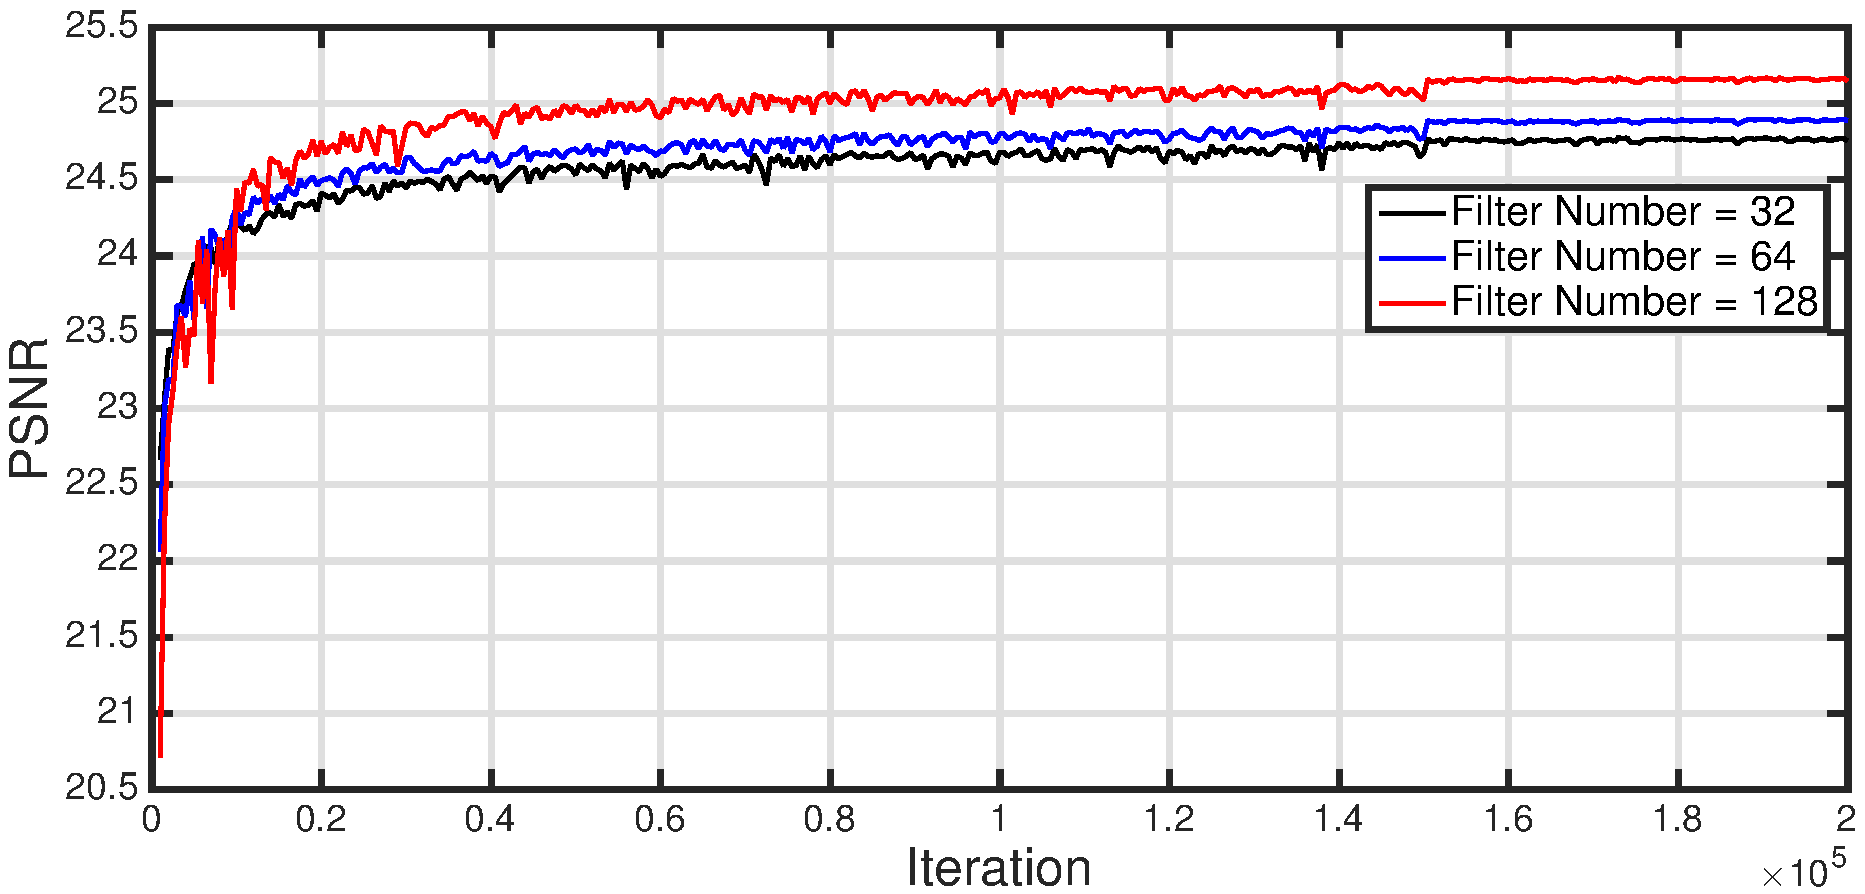
\includegraphics[width=0.48\textwidth]{filternum}
\caption{The PSNR values on the validation set during training with different number of filters.}
\label{fig9}
\end{figure}

For the experiments on filter size, we set the filter number to be 64, training patch
size as 50$\times$50, skip connection step size as 2.

Filter size of 3$\times$3,
5$\times$5, 7$\times$7, 9$\times$9 are tested. Figure \ref{fig10} show the PSNR values
on the validation set while training. It is clear that larger filter size leads to
better performance. Different from high-level tasks~\cite{DBLP:conf/eccv/ZeilerF14,
DBLP:journals/corr/SermanetEZMFL13,DBLP:journals/corr/SimonyanZ14a} which favor smaller
filter sizes, larger filter size tends to obtain better performance in low-level image
restoration applications.

However, there  may  exist a bottle neck  as  the performance
of 9$\times$9 is almost as the same as 7$\times$7 in our experiments. The reason may be
that for high-level tasks, the networks have to learn image abstraction for classification, which is usually
very different from the input pixels. Larger filter size may result in larger respective fields,
but also made the networks more difficult to train and converge to a poor optimum. Using
smaller filter size is mainly beneficial for convergence in such complex mappings.

In contrast, for low-level image restoration, the training is not as difficult as that in high-level
applications since only a bias is needed to be learned to revise the corrupted pixel.
In this situation, utilizing neighborhood information in the mapping stage is more important,
since the desired value for a pixel should be predicted from its neighbor pixels.
However, using larger filter size inevitably increases the complexity (e.g., filter
size of 9$\times$9 is 9 times more complex as 3$\times$3) and training time.

\begin{figure}[t!]
\centering
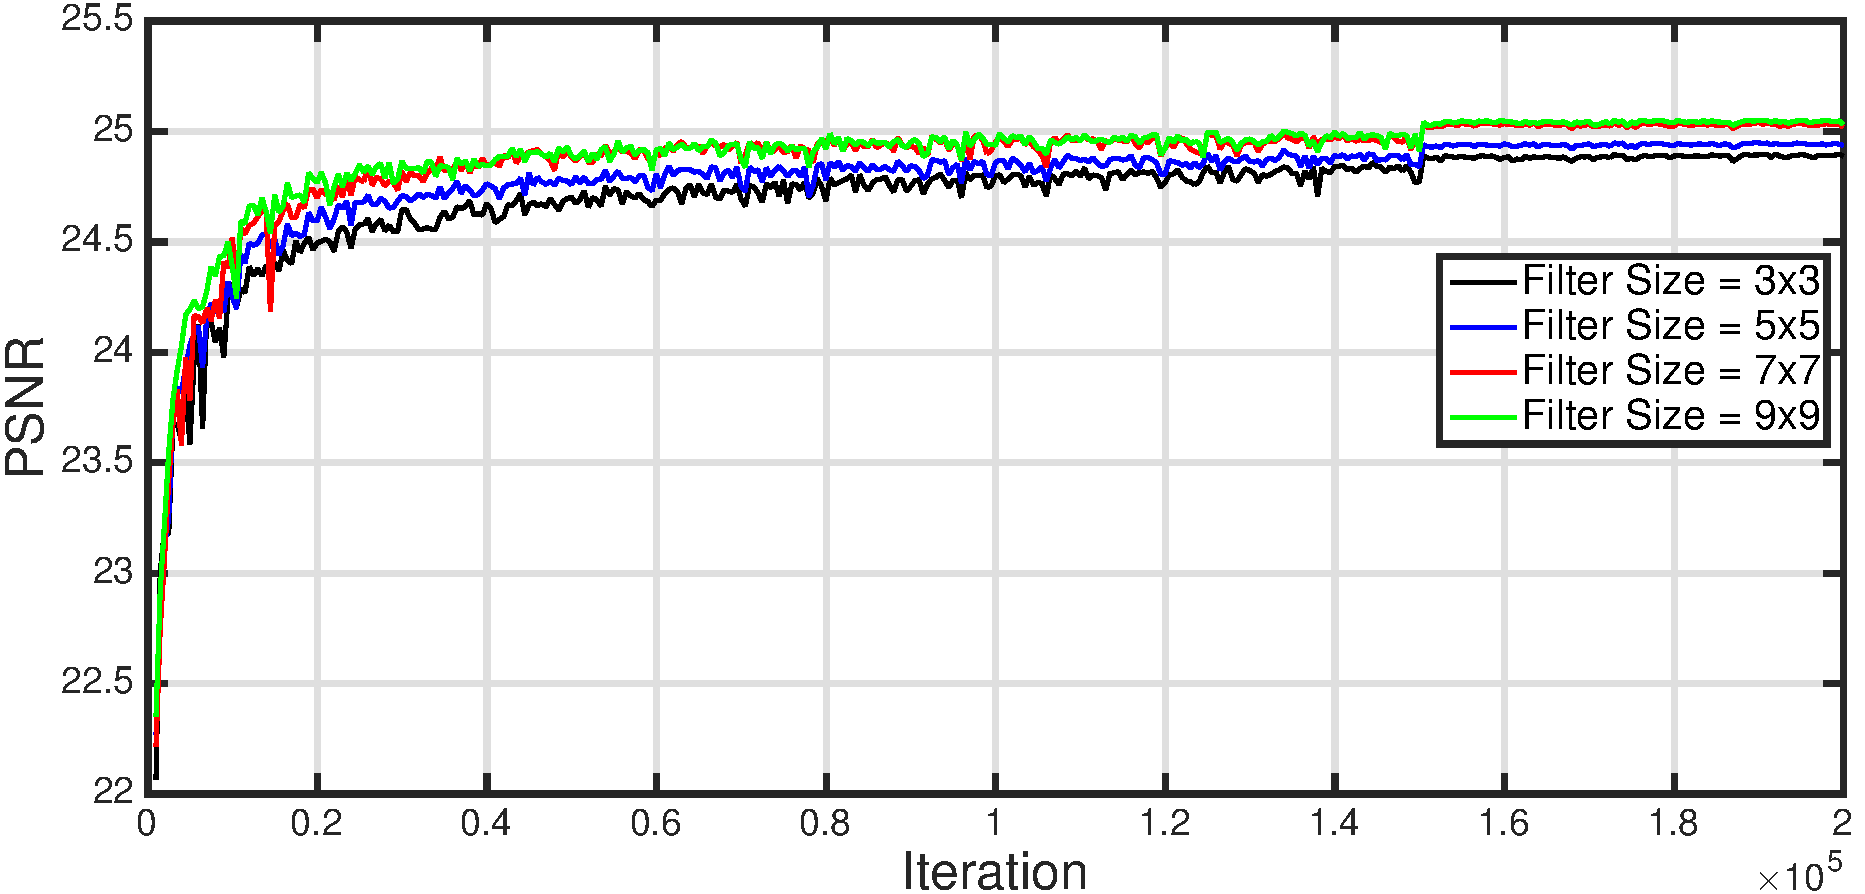
\includegraphics[width=0.48\textwidth]{filtersize}
\caption{The PSNR values on the validation set during training with different size of filters.}
\label{fig10}
\end{figure}

For the training patch size, we set the filter number to be 64, filter size as 3$\times$3,
skip connection step size as 2. Then we test different training patch sizes of 25$\times$25,
50$\times$50, 75$\times$75, 100$\times$100, as shown in Figure \ref{fig11}.

Better
performance is achieved with larger training patch size. The reason can be two folds.
First of all, since the network essentially performs pixel-wise prediction, if the number
of training patches are the same, larger size of training patch results in more pixels
to be used, which is equivalent to using more training data. Secondly, the corruptions
in image restoration tasks can be described as some types of latent distributions. Larger
size of training patch contains more pixels that better capture the latent distributions
to be learned, which consequently helps the network to fit the corruptions better.

\begin{figure}[b!]
\centering
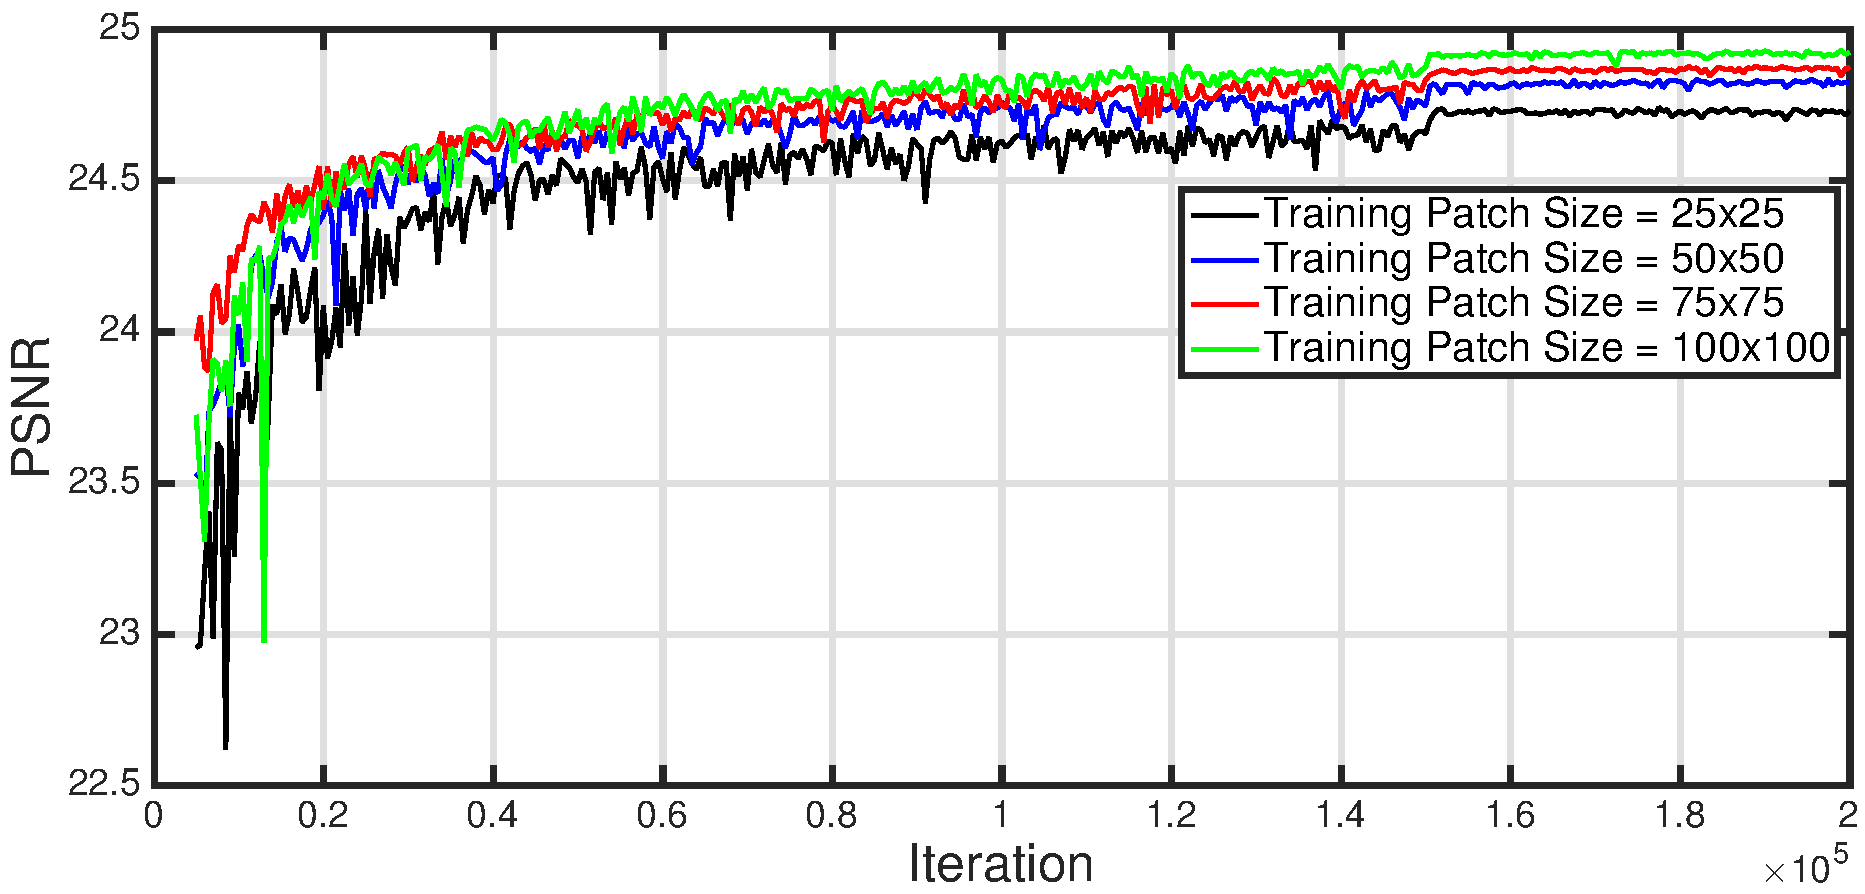
\includegraphics[width=0.48\textwidth]{patchsize}
\caption{The PSNR values on the validation set during training with different size of training patch.}
\label{fig11}
\end{figure}


As we can see, the ``width" of the network is as crucial as the ``depth" in training
a network with satisfactory image restoration performance. However, one should always make a
trade-off between the performance and speed.

We also provide the experiments of different step sizes of shortcuts, as shown in
Figure \ref{fig7}. A smaller step size of shortcuts achieves better performance than
a larger one. We believe that a smaller step size of shortcuts makes it easier
to back-propagate the gradient to bottom layers, thus tackle the gradient vanishing
issue better. Meanwhile, a small step size of shortcuts essentially passes more direct information.

\begin{figure}[htb!]
\centering
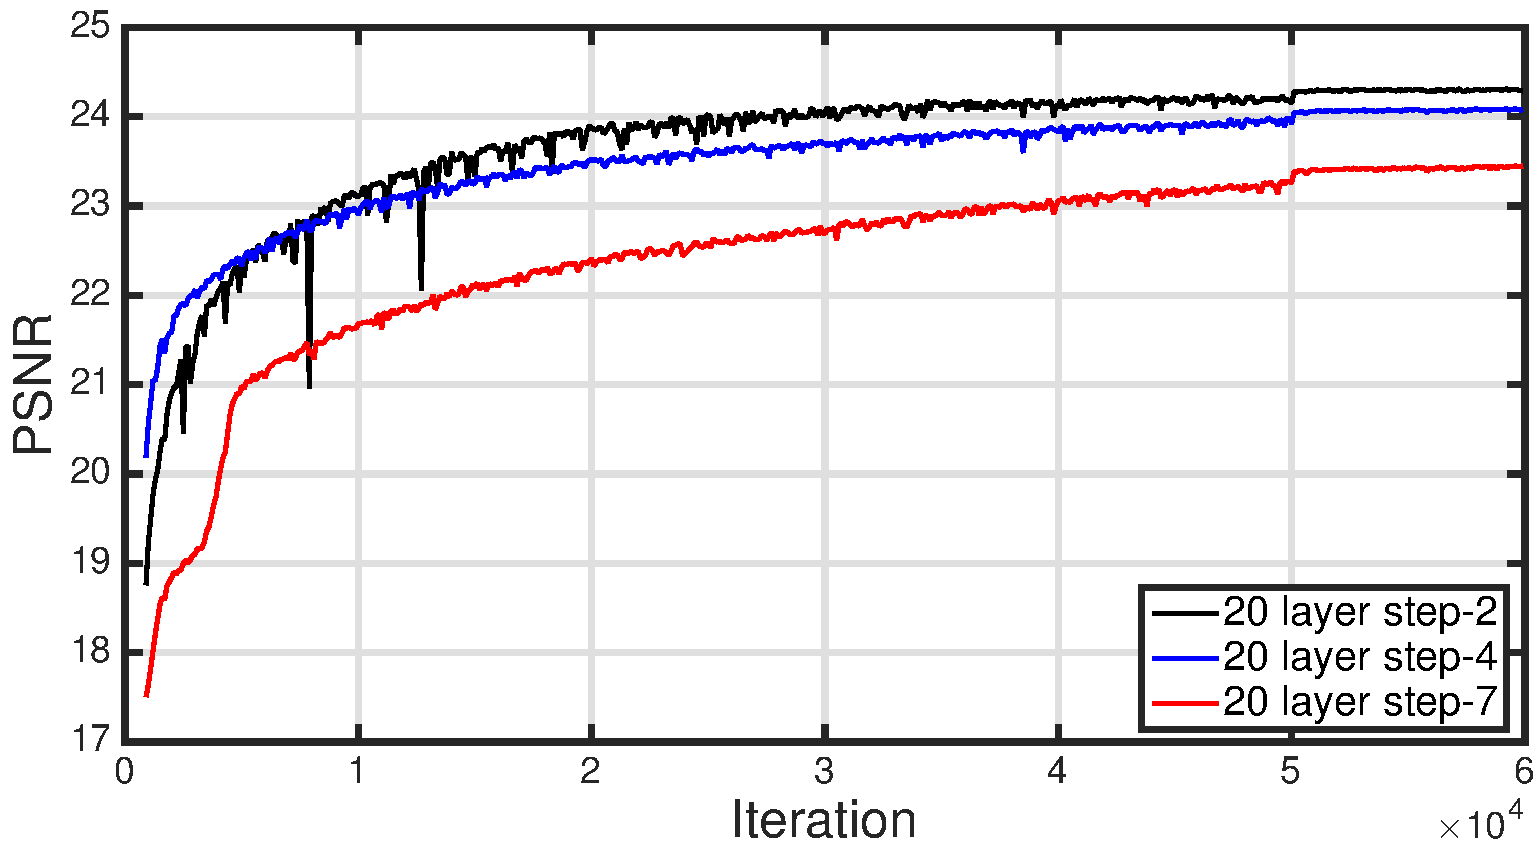
\includegraphics[width=0.48\textwidth]{block-size-psnr}
\caption{The PSNR values on the validation set during training.}
\label{fig7}
\end{figure}







\subsection{Image denoising}

Image denoising experiments are performed on two datasets: 14 common benchmark images
~\cite{DBLP:conf/iccv/XuZZZF15,DBLP:conf/iccv/ChenZY15,DBLP:conf/cvpr/LiuXZG15,
DBLP:conf/cvpr/GuZZF14}, as show in Figure \ref{fig12} and the BSD dataset.

As a common
experimental setting in the literature, additive Gaussian noises with zero mean and
standard deviation $\sigma$ are added to the image to test the performance of denoising
methods. In this paper we test noise level $\sigma$ of 10, 30, 50 and 70. BM3D
~\cite{DBLP:journals/tip/DabovFKE07}, NCSR~\cite{DBLP:journals/tip/DongZSL13}, EPLL
~\cite{DBLP:conf/iccv/ZoranW11}, PCLR~\cite{DBLP:conf/iccv/ChenZY15}, PGPD~\cite{DBLP:conf/iccv/XuZZZF15}
and WMMN~\cite{DBLP:conf/cvpr/GuZZF14} are compared with our method. For these methods,
we use the source code released by their authors and test on the images with their default parameters.

\begin{figure}
\centering
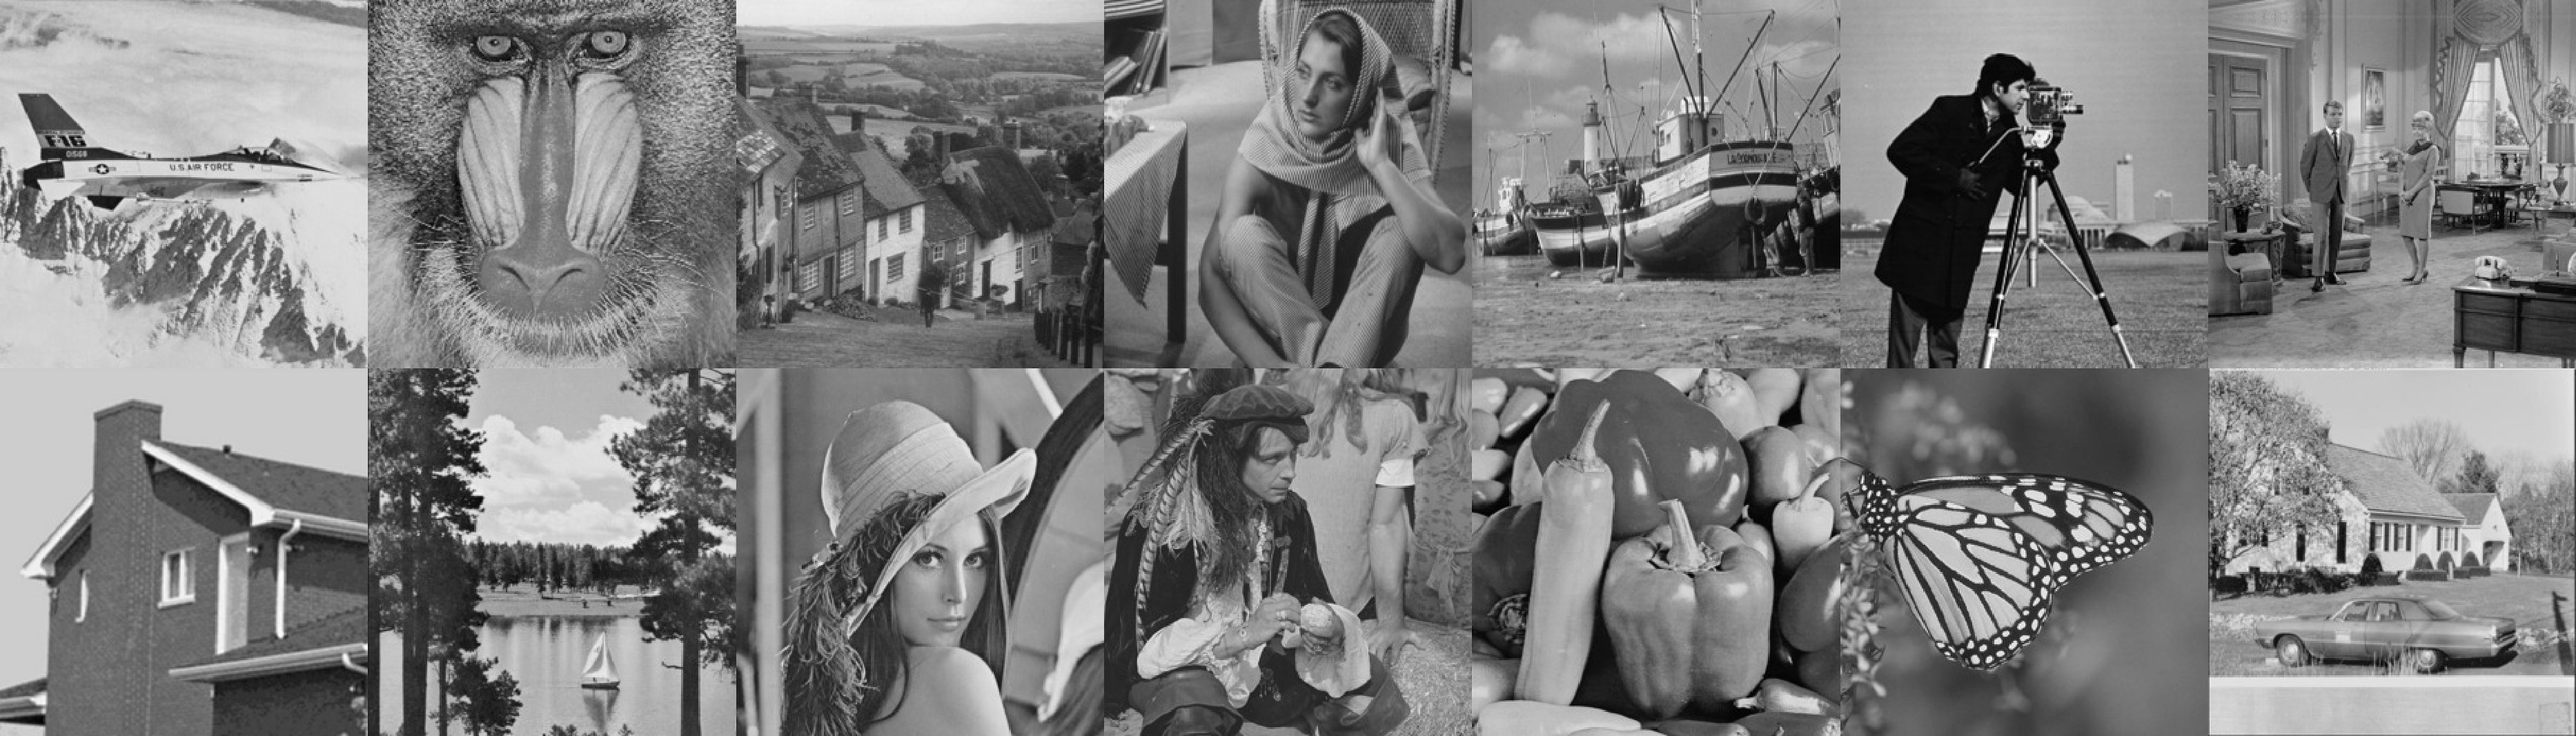
\includegraphics[width=0.48\textwidth]{test}
\caption{The 14 testing images for denoising.}
\label{fig12}
\end{figure}


{\bf{Evaluation on the 14 images}}  Table \ref{table2} presents the PSNR and SSIM
results of $\sigma$ 10, 30, 50, and 70. We can make some observations from the results.
First of all, the 10 layer convolutional and deconvolutional network has already achieved
better results than the state-of-the-art methods, which demonstrates that combining
convolution and deconvolution for denoising works well, even without any skip connections.

Moreover, when the network goes deeper, the skip connections proposed in this paper help to
achieve even better denoising performance, which exceeds the existing best method WNNM
~\cite{DBLP:conf/cvpr/GuZZF14} by 0.32dB, 0.43dB, 0.49dB and 0.51dB on noise levels of $\sigma$
being 10, 30, 50 and 70 respectively. While WNNM is only slightly better than the second
best existing method PCLR~\cite{DBLP:conf/iccv/ChenZY15} by 0.01dB, 0.06dB, 0.03dB and 0.01dB
respectively, which shows the large improvement of our model.

Last, we can observe that the
more complex the noise is, the more improvement our model achieves than other methods.
Similar observations can be made on the evaluation of SSIM.

\begin{table*}[htb!]
\centering
%
\caption{Average PSNR and SSIM results of $\sigma$ 10, 30, 50, 70 on 14 images.}
\begin{tabular}{c|c c c c c c c c c} \hline
              &\multicolumn{9}{c}{PSNR}            \\ \hline
              &BM3D   &EPLL   &NCSR   &PCLR   &PGPD   &WNNM   &RED10  &RED20  &RED30          \\ \hline
  $\sigma=10$ &34.18  &33.98  &34.27  &34.48  &34.22  &34.49  &34.62  &34.74  &\textbf{34.81} \\ \hline
  $\sigma=30$ &28.49  &28.35  &28.44  &28.68  &28.55  &28.74  &28.95  &29.10  &\textbf{29.17} \\ \hline
  $\sigma=50$ &26.08  &25.97  &25.93  &26.29  &26.19  &26.32  &26.51  &26.72  &\textbf{26.81} \\ \hline
  $\sigma=70$ &24.65  &24.47  &24.36  &24.79  &24.71  &24.80  &24.97  &25.23  &\textbf{25.31} \\ \hline
              &\multicolumn{9}{c}{SSIM}            \\ \hline
  $\sigma=10$ &0.9339 &0.9332 &0.9342 &0.9366 &0.9309 &0.9363 &0.9374 &0.9392 &\textbf{0.9402} \\ \hline
  $\sigma=30$ &0.8204 &0.8200 &0.8203 &0.8263 &0.8199 &0.8273 &0.8327 &0.8396 &\textbf{0.8423} \\ \hline
  $\sigma=50$ &0.7427 &0.7354 &0.7415 &0.7538 &0.7442 &0.7517 &0.7571 &0.7689 &\textbf{0.7733} \\ \hline
  $\sigma=70$ &0.6882 &0.6712 &0.6871 &0.6997 &0.6913 &0.6975 &0.7012 &0.7177 &\textbf{0.7206} \\ \hline
\end{tabular}
\label{table2}
\end{table*}



{\bf{Evaluation on BSD200}} For the BSD dataset, 300 images are used for training and
the remaining 200 images are used for denoising to show more experimental results.
For efficiency, we convert the images to gray-scale and resize them to smaller images.
Then all the methods are run on the dataset to get average PSNR and SSIM results of
$\sigma$ 10, 30, 50, and 70, as shown in Table \ref{table3}. For existing methods,
their denoising performance does not differ much, while our model achieves 0.38dB,
0.47dB, 0.49dB and 0.42dB higher of PSNR over WNNM \cite{DBLP:conf/cvpr/GuZZF14}.

\begin{table*}[htb!]
\centering
%
\caption{Average PSNR and SSIM results of $\sigma$ 10, 30, 50, 70 on BSD.}
\begin{tabular}{ c|c c c c c c c c c } \hline
			  &\multicolumn{9}{c}{PSNR}            \\ \hline
              &BM3D   &EPLL   &NCSR   &PCLR   &PGPD   &WNNM   &RED10  &RED20  &RED30 \\ \hline
  $\sigma=10$ &33.01  &33.01  &33.09  &33.30  &33.02  &33.25  &33.49  &33.59  &\textbf{33.63} \\ \hline
  $\sigma=30$ &27.31  &27.38  &27.23  &27.54  &27.33  &27.48  &27.79  &27.90  &\textbf{27.95} \\ \hline
  $\sigma=50$ &25.06  &25.17  &24.95  &25.30  &25.18  &25.26  &25.54  &25.67  &\textbf{25.75} \\ \hline
  $\sigma=70$ &23.82  &23.81  &23.58  &23.94  &23.89  &23.95  &24.13  &24.33  &\textbf{24.37} \\ \hline
              &\multicolumn{9}{c}{SSIM}            \\ \hline
  $\sigma=10$ &0.9218 &0.9255 &0.9226 &0.9261 &0.9176 &0.9244 &0.9290 &0.9310 &\textbf{0.9319} \\ \hline
  $\sigma=30$ &0.7755 &0.7825 &0.7738 &0.7827 &0.7717 &0.7807 &0.7918 &0.7993 &\textbf{0.8019} \\ \hline
  $\sigma=50$ &0.6831 &0.6870 &0.6777 &0.6947 &0.6841 &0.6928 &0.7032 &0.7117 &\textbf{0.7167} \\ \hline
  $\sigma=70$ &0.6240 &0.6168 &0.6166 &0.6336 &0.6245 &0.6346 &0.6367 &0.6521 &\textbf{0.6551} \\ \hline
\end{tabular}
\label{table3}
\end{table*}



{\bf{Blind denoising}} We also perform blind denoising to show the superior performance
of our network. In blind denoising, the training set consists of image patches of different
levels of noises, and a 30-layer network is trained on this training set. In the testing
phase, we test noisy images with $\sigma$ of 10, 30, 50 and 70 using this model. The evaluation
results are shown in Table \ref{table4}. Although training with different levels of corruption,
we can observe that the performance of our network degrades comparing to the case in which
using separate models for denoising. This is reasonable because the network has to fit much
more complex mappings. However, it still beats the existing methods. For PSNR evaluation,
our blind denoising model achieves the same performance as WNNM  \cite{DBLP:conf/cvpr/GuZZF14}
on $\sigma=10$, and outperforms
WNNM \cite{DBLP:conf/cvpr/GuZZF14} by
 0.35dB, 0.43dB and 0.40dB on $\sigma$ = 30, 50 and 70 respectively, which is still
marginal improvements. For SSIM evaluation, our network is 0.0005, 0.0141, 0.0199 and 0.0182
higher than WNNM. The performance improvement is more obvious on BSD dataset. The 30-layer
network outperforms the second best method WNNM \cite{DBLP:conf/cvpr/GuZZF14} by
 0.13dB, 0.4dB, 0.43dB, 0.41dB for
PSNR and 0.0036, 0.0173, 0.0191, 0.0198 for SSIM.

\begin{table}[b!]
\centering
%
\caption{Average PSNR and SSIM results for image denoising using a single 30-layer network.}
\begin{tabular}{ c|c c c c } \hline
       &\multicolumn{4}{c}{14 images}                     \\ \hline
       &$\sigma=10$ &$\sigma=30$ &$\sigma=50$ &$\sigma=70$ \\ \hline
  PSNR &34.49       &29.09       &26.75       &25.20       \\ \hline
  SSIM &0.9368      &0.8414      &0.7716      &0.7157      \\ \hline
     &\multicolumn{4}{c}{BSD200}                          \\ \hline
       &$\sigma=10$ &$\sigma=30$ &$\sigma=50$ &$\sigma=70$ \\ \hline
  PSNR &33.38       &27.88       &25.69       &24.36       \\ \hline
  SSIM &0.9280      &0.7980      &0.7119      &0.6544      \\ \hline
\end{tabular}
\label{table4}
\end{table}

{\bf{Visual results}} Some visual results are shown in Figure \ref{fig13}. We highlight
some details of the clean image and the recovered ones by different methods. The first
observation is that our method better recovers the image details, as we can see from the
third and fourth rows, which is due to the high PSNR we achieve by minimizing the pixel-wise
Euclidean loss.

 Moreover, we can observe from the first and second rows that our network
obtains more visually smooth results than other methods. This may due to the testing
strategy which average the output of different orientations.

\begin{figure*}
\centering
\subfigure{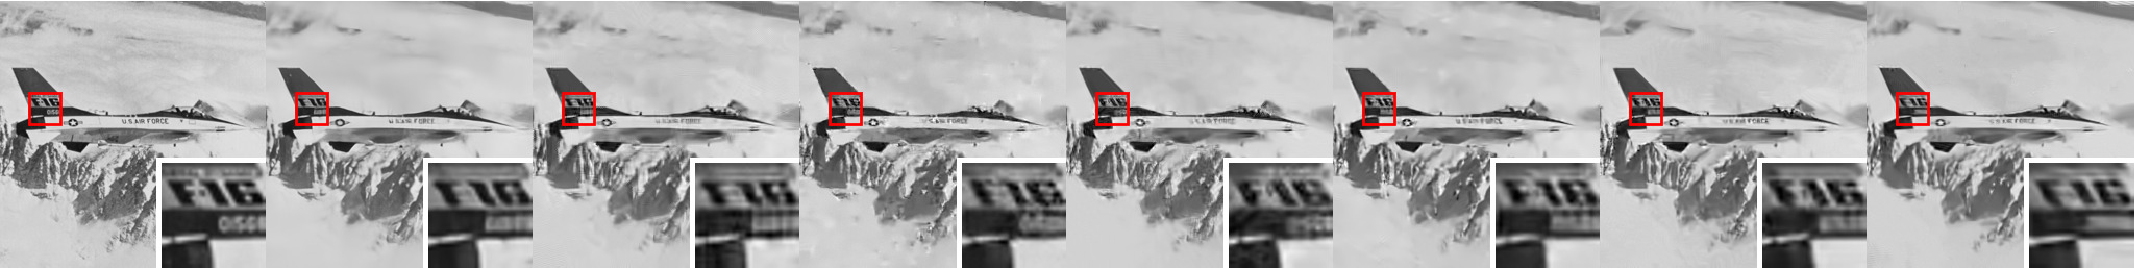
\includegraphics[width=1\textwidth]{30-1} }
\subfigure{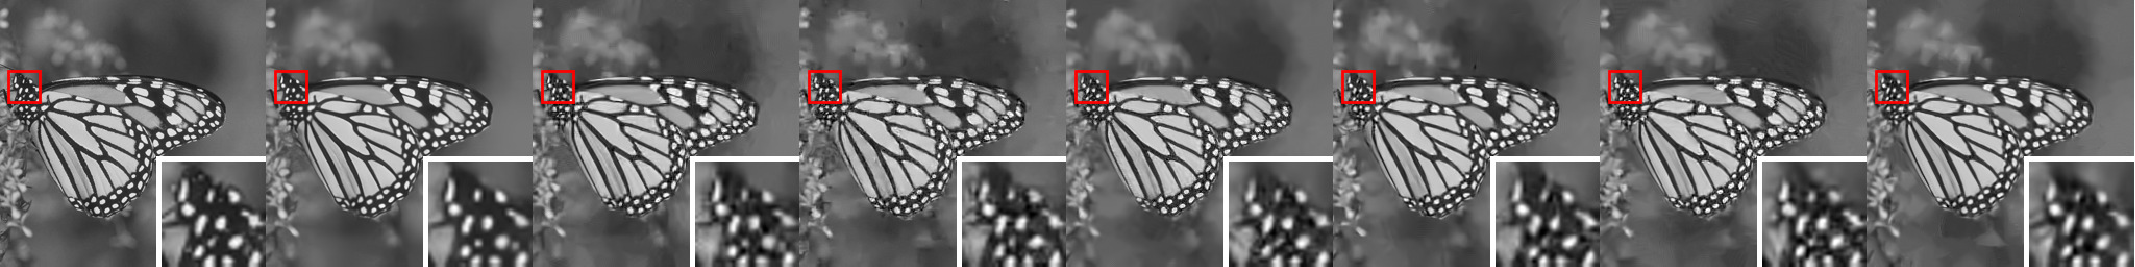
\includegraphics[width=1\textwidth]{30-2} }
\subfigure{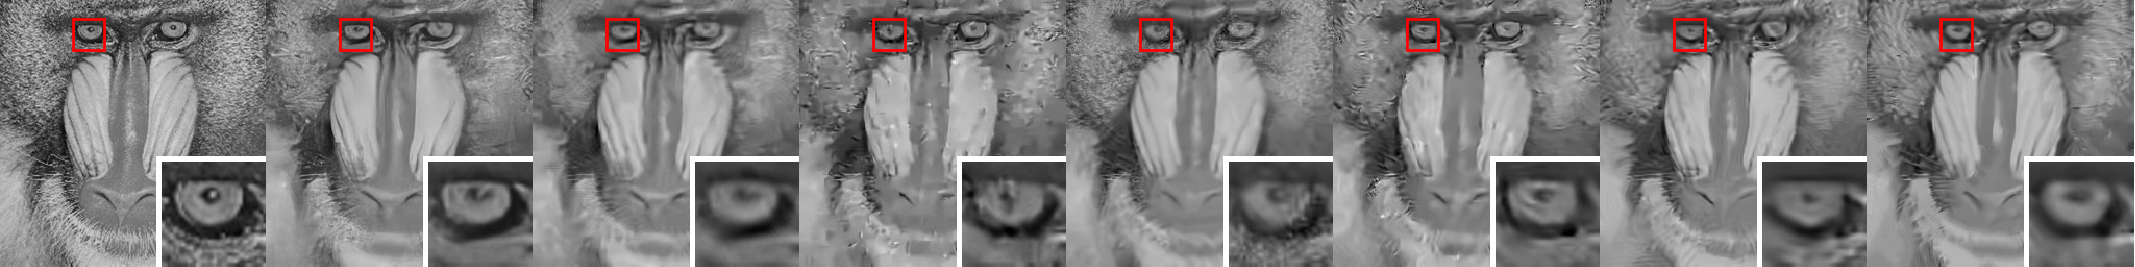
\includegraphics[width=1\textwidth]{50-1} }
\subfigure{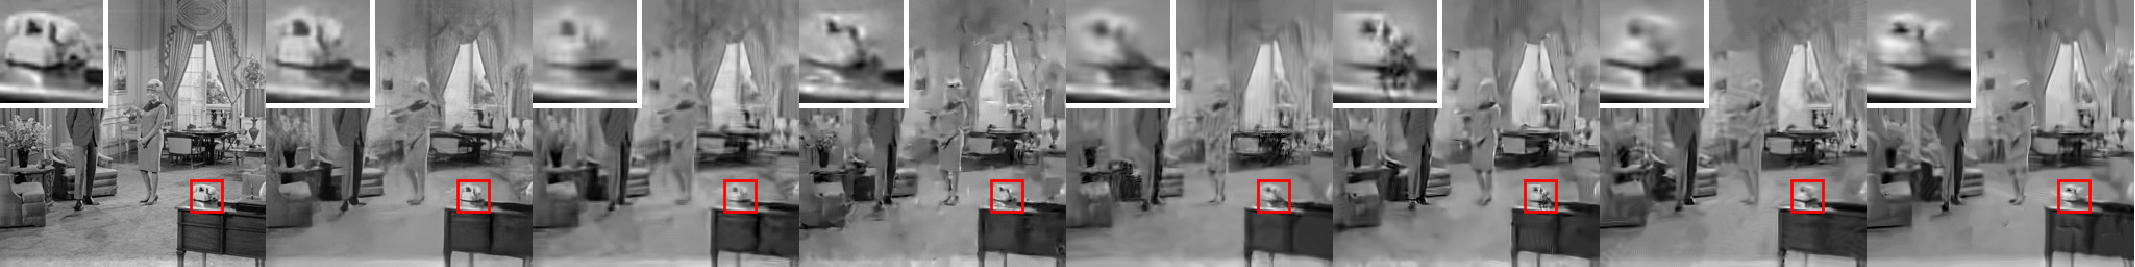
\includegraphics[width=1\textwidth]{50-2} }
\caption{Visual results of image denoising. Images from left to right column are:
clean image; the recovered image of RED30, BM3D, EPLL, NCSR, PCLR, PGPD, WNNM.}
\label{fig13}
\end{figure*}





\subsection{Image super-resolution}

For super-resolution, The high-resolution image is first down-sampled with scaling
factor parameters of 2, 3 and 4 respectively. Since the size of the input and output of our
network are the same, we up-sample the low-resolution image to its original size as
the input of our network. We compare our network with SRCNN~\cite{DBLP:journals/pami/DongLHT16},
NBSRF~\cite{DBLP:conf/iccv/SalvadorP15}, CSCN~\cite{DBLP:conf/iccv/WangLYHH15},
CSC~\cite{DBLP:conf/iccv/GuZXMFZ15}, TSE~\cite{DBLP:conf/cvpr/HuangSA15} and ARFL+
~\cite{DBLP:conf/cvpr/SchulterLB15} on three dataset: Set5, Set14 and BSD100.

The results of the compared methods are either cited from their original papers or obtained
using the released source code by the authors.


{\bf{Evaluation on Set 5}} The evaluation on Set5 is shown in Table \ref{table5}.
In general, our 10-layer network already outperforms the compared methods, and we
achieve better performance with deeper networks.

 The second best method is CSCN, which
is also a recently proposed neural network based method. Compared to CSCN, our
30-layer network exceeds it by 0.52dB, 0.56dB, 0.47dB on PSNR and 0.0032, 0.0063,
0.0094 on SSIM respectively.

The larger scaling parameter is, the better improvement
our method can make, which demonstrates that our network is better at fitting
complex corruptions than other methods.

\begin{table*}[htb!]
\centering
%
\caption{Average PSNR and SSIM results of scaling 2, 3 and 4 on Set5.}
\begin{tabular}{ c|c c c c c c c c c }  \hline
              &\multicolumn{9}{c }{PSNR}            \\ \hline
           &SRCNN  &NBSRF  &CSCN   &CSC    &TSE    &ARFL+   &RED10    &RED20   &RED30           \\ \hline
  $s = 2$  &36.66  &36.76  &37.14  &36.62  &36.50  &36.89   &37.43    &37.62   &\textbf{37.66}  \\ \hline
  $s = 3$  &32.75  &32.75  &33.26  &32.66  &32.62  &32.72   &33.43    &33.80   &\textbf{33.82}  \\ \hline
  $s = 4$  &30.49  &30.44  &31.04  &30.36  &30.33  &30.35   &31.12    &31.40   &\textbf{31.51}  \\ \hline
              &\multicolumn{9}{c }{SSIM}            \\ \hline
  $s = 2$  &0.9542 &0.9552 &0.9567 &0.9549 &0.9537 &0.9559  &0.9590   &0.9597  &\textbf{0.9599} \\ \hline
  $s = 3$  &0.9090 &0.9104 &0.9167 &0.9098 &0.9094 &0.9094  &0.9197   &0.9229  &\textbf{0.9230} \\ \hline
  $s = 4$  &0.8628 &0.8632 &0.8775 &0.8607 &0.8623 &0.8583  &0.8794   &0.8847  &\textbf{0.8869} \\ \hline
\end{tabular}
\label{table5}
\end{table*}

{\bf{Evaluation on Set 14}} The evaluation on Set14 is shown in Table \ref{table6}.
The improvement on Set14 in not as significant as that on Set5, but we can still
observe that the 30-layer network achieves higher PSNR and SSIM than the second
best CSCN for 0.23dB, 0.06dB, 0.1dB and 0.0049, 0.0070, 0.0098. The performance
on 10-layer, 20-layer and 30-layer RED-Net also does not improve that much as on
Set5, which may imply that Set14 is more difficult to perform image super-resolution.

\begin{table*}[htb!]
\centering
%
\caption{Average PSNR and SSIM results of scaling 2, 3 and 4 on Set14.}
\begin{tabular}{c|c c c c c c c c c}  \hline
              &\multicolumn{9}{c}{PSNR}            \\ \hline
           &SRCNN  &NBSRF  &CSCN   &CSC    &TSE    &ARFL+   &RED10    &RED20   &RED30           \\ \hline
  $s = 2$  &32.45  &32.45  &32.71  &32.31  &32.23  &32.52   &32.77    &32.87   &\textbf{32.94}  \\ \hline
  $s = 3$  &29.30  &29.25  &29.55  &29.15  &29.16  &29.23   &29.42    &29.61   &\textbf{29.61}  \\ \hline
  $s = 4$  &27.50  &27.42  &27.76  &27.30  &27.40  &27.41   &27.58    &27.80   &\textbf{27.86}  \\ \hline
              &\multicolumn{9}{c}{SSIM}            \\ \hline
  $s = 2$  &0.9067 &0.9071 &0.9095 &0.9070 &0.9036 &0.9074 &0.9125    &0.9138  &\textbf{0.9144} \\ \hline
  $s = 3$  &0.8215 &0.8212 &0.8271 &0.8208 &0.8197 &0.8201 &0.8318    &0.8343  &\textbf{0.8341} \\ \hline
  $s = 4$  &0.7513 &0.7511 &0.7620 &0.7499 &0.7518 &0.7483 &0.7654    &0.7697  &\textbf{0.7718} \\ \hline
\end{tabular}
\label{table6}
\end{table*}

{\bf{Evaluation on BSD 100}} We also evaluate super-resolution results on BSD100,
as shown in Table \ref{table7}. The overall results are very similar than those on Set5.
CSCN is still the second best method and outperforms other compared methods by large
margin, but its performance is not as good as our 10-layer network. Our deeper networks
obtain performance gains. Compared to CSCN, the 30-layer network achieves higher
PSNR for 0.45dB, 0.38dB, 0.29dB and higher SSIM for 0.0066, 0.0084, 0.0099.

\begin{table*}[htb!]
\centering
%
\caption{Average PSNR and SSIM results of scaling 2, 3 and 4 on BSD100}
\begin{tabular}{c|c c c c c c c c c}  \hline
              &\multicolumn{9}{c}{PSNR}            \\ \hline
           &SRCNN  &NBSRF  &CSCN   &CSC    &TSE    &ARFL+  &RED10  &RED20   &RED30           \\ \hline
  $s = 2$  &31.36  &31.30  &31.54  &31.27  &31.18  &31.35  &31.85  &31.95   &\textbf{31.99}  \\ \hline
  $s = 3$  &28.41  &28.36  &28.58  &28.31  &28.30  &28.36  &28.79  &28.90   &\textbf{28.93}  \\ \hline
  $s = 4$  &26.90  &26.88  &27.11  &26.83  &26.85  &26.86  &27.25  &27.35   &\textbf{27.40}  \\ \hline
              &\multicolumn{9}{c}{SSIM}            \\ \hline
  $s = 2$  &0.8879 &0.8876 &0.8908 &0.8876 &0.8855 &0.8885 &0.8953 &0.8969  &\textbf{0.8974} \\ \hline
  $s = 3$  &0.7863 &0.7856 &0.7910 &0.7853 &0.7843 &0.7851 &0.7975 &0.7993  &\textbf{0.7994} \\ \hline
  $s = 4$  &0.7103 &0.7110 &0.7191 &0.7101 &0.7108 &0.7091 &0.7238 &0.7268  &\textbf{0.7290} \\ \hline
\end{tabular}
\label{table7}
\end{table*}


{\bf{Comparisons with VDSR~\cite{DBLP:journals/corr/KimLL15b}
and DRCN~\cite{DBLP:journals/corr/KimLL15a}}}
Concurrent to our work \cite{NIPS2016Mao}, networks~\cite{DBLP:journals/corr/KimLL15b,DBLP:journals/corr/KimLL15a}
which incorporate residual learning for image super-resolution are proposed.
In \cite{DBLP:journals/corr/KimLL15b}, a fully convolutional network termed  VDSR
is proposed to learn the residual image for image super-resolution.
The loss layer takes three inputs: residual estimate, low-resolution input and
ground truth high-resolution image, and Euclidean loss is computed between the
reconstructed image (the sum of network input and output) and ground truth.
DRCN~\cite{DBLP:journals/corr/KimLL15a} proposed to use a recursive convolutional block,
which does not increase the number of parameters while increasing the depth of the network.
To ease the training, firstly each recursive layer is supervised to reconstruct the
target high-resolution image (HR). The second proposal is to use a skip-connection
from input to the output. During training, the network has $D$ outputs,
in which the $d$th output $y_d = x + {\rm Rec}(H_d)$. $x$ is the input low-resolution image,
${\rm Rec}()$ denotes the reconstruction layer and $H_d$ is the output of $d$th recursive layer.
The final loss includes three parts: (a) the Euclidean loss between the ground truth and each $y_d$;
(b) the Euclidean loss between the ground truth and the weighted sum of all $y_d$; and
(c) the L2 regularization on the network weights. Although skip connections are used in our network,
VDSR and DCRN to perform identity mapping, their differences are significant.

Firstly, {\em both VDSR and DRCN use one path of connections between the input and output,
which actually models the corruptions.}  In VDSR, the network itself is standard fully convolutional.
DRCN uses recursive convolutional layers that lead to multiple losses, which is different from VDSR.
The skip connections in VDSR and DRCN model the super-resolution problem as learning the residual image,
which actually learns the corruption as in image restoration. In other words,
the residual learning is only conducted in the input-output level (low-resolution and high-resolution images)
in VDSR and DRCN. In contrast, {\em  our network uses multiple skip connections that divide the
network into multiple blocks for residual learning}. Secondly, our skip connections pass
image abstraction of different levels from multiple convolutional layers forwardly.
No such information is used in VDSR and DRCN. In VDSR and DRCN,
the skip connection only pass the input image. However, in our network,
different levels of image abstraction are obtained after the convolutional layers,
and they are passed to the deconvolutional layers for reconstruction. At last,
our skip connections help to back-propagate gradients in different layers. In VDSR and DCRN,
the skip connections do not involve in back-propagating gradients since they connect the input and output,
and there are no weights to be updated for the input low-resolution image.
The image super-resolution comparisons of VDSR, DRCN and our network on Set5,
Set14 and BSD100 are provided in Table~\ref{table11}.




\begin{table*}[htb!]
\centering
%
\caption{Comparisons between RED30 (ours), VDSR \cite{DBLP:journals/corr/KimLL15b}
and DRCN \cite{DBLP:journals/corr/KimLL15a}: Average PSNR and SSIM results of scaling 2, 3 and 4 on Set5, Set14 and BSD100.}
\begin{tabular}{ c|c|c c c }  \hline
Dataset                 &Scale        &VDSR  (PSNR/SSIM)    &DRCN (PSNR/SSIM)    &RED30 (PSNR/SSIM)  \\ \hline
\multirow{3}{*}{Set5}   &$\times$2    &37.53/0.9587       &37.63/0.9588       &\textbf{37.66}/\textbf{0.9599}      \\
                        &$\times$3    &33.66/0.9213       &33.82/0.9226       &\textbf{33.82}/\textbf{0.9230}      \\
                        &$\times$4    &31.35/0.8838       &\textbf{31.53}/0.8854       &31.51/\textbf{0.8869}      \\ \hline\hline
\multirow{3}{*}{Set14}  &$\times$2    &33.03/0.9124       &\textbf{33.04}/0.9118       &32.94/\textbf{0.9144}      \\
                        &$\times$3    &\textbf{29.77}/0.8314       &29.76/0.8311       &29.61/\textbf{0.8341}      \\
                        &$\times$4    &28.01/0.7674       &\textbf{28.02}/0.7670       &27.86/\textbf{0.7718}      \\ \hline\hline
\multirow{3}{*}{BSD100} &$\times$2    &31.90/0.8960       &31.85/0.8942       &\textbf{31.99}/\textbf{0.8974}      \\
                        &$\times$3    &28.82/0.7976       &28.80/0.7963       &\textbf{28.93}/\textbf{0.7994}      \\
                        &$\times$4    &27.29/0.7251       &27.23/0.7233       &\textbf{27.40}/\textbf{0.7290}      \\ \hline
\end{tabular}
\label{table11}
\end{table*}




{\bf{Blind super-resolution}} The results of blind super-resolution are shown in
Table \ref{table8}. Among the compared methods, CSCN can also deal with different
scaling parameters by repeatedly enlarging the image by a smaller scaling factor.

 Our method is
different from CSCN. Given a low-resolution image as input and the output size,
we first up-sample the input image to the desired size, resulting in an image with
poor details. Then the image is fed into our network. The output is an image of the
same size with fine details. The training set consists of image patches of different
scaling parameters and a single model is trained. Except that CSCN works slightly
better on Set 14 with scaling factors 3 and 4, our network  outperforms the existing methods,
showing that our network works much better in image super-resolution even using only
one single model to deal with complex corruptions.

\begin{table}[htb!]
\centering
%
\caption{Average PSNR and SSIM results for image super-resolution using a single 30 layer network.}
\begin{tabular}{c|c c c } \hline
       &\multicolumn{3}{c}{Set5}     \\ \hline
       &$s = 2$  &$s = 3$  &$s = 4$  \\ \hline
  PSNR &37.56    &33.70    &31.33    \\ \hline
  SSIM &0.9595   &0.9222   &0.8847   \\ \hline
       &\multicolumn{3}{c}{Set14}    \\ \hline
       &$s = 2$  &$s = 3$  &$s = 4$  \\ \hline
  PSNR &32.81    &29.50    &27.72    \\ \hline
  SSIM &0.9135   &0.8334   &0.7698   \\ \hline
       &\multicolumn{3}{c}{BSD100}   \\ \hline
       &$s = 2$  &$s = 3$  &$s = 4$  \\ \hline
  PSNR &31.96    &28.88    &27.35    \\ \hline
  SSIM &0.8972   &0.7993   &0.7276   \\ \hline
\end{tabular}
\label{table8}
\end{table}


{\bf{Visual results}} Some visual results in grey-scale images are shown in Figure \ref{fig14}.
Note that it is straightforward to perform super-resolution on color images.

We can observe from
the second and third rows that our network is better at obtaining high resolution edges
and text. Meanwhile, our results seem much more smooth than others. For faces such as
the fourth row, out network still obtains better visually results.

\begin{figure*}
\centering
\subfigure{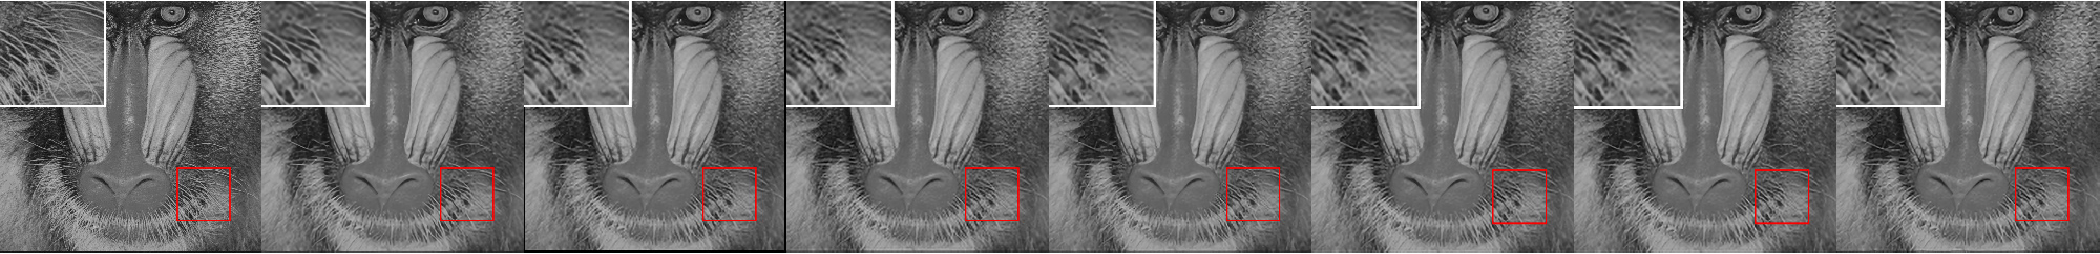
\includegraphics[width=1\textwidth]{3-1} }
\subfigure{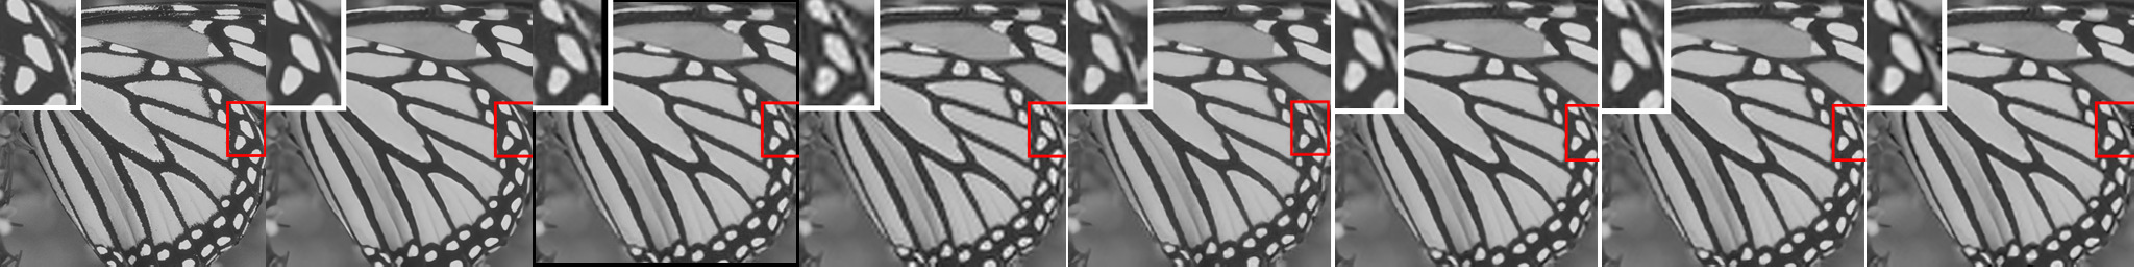
\includegraphics[width=1\textwidth]{3-2} }
\subfigure{
\includegraphics[width=1\textwidth]{3-3} }
\subfigure{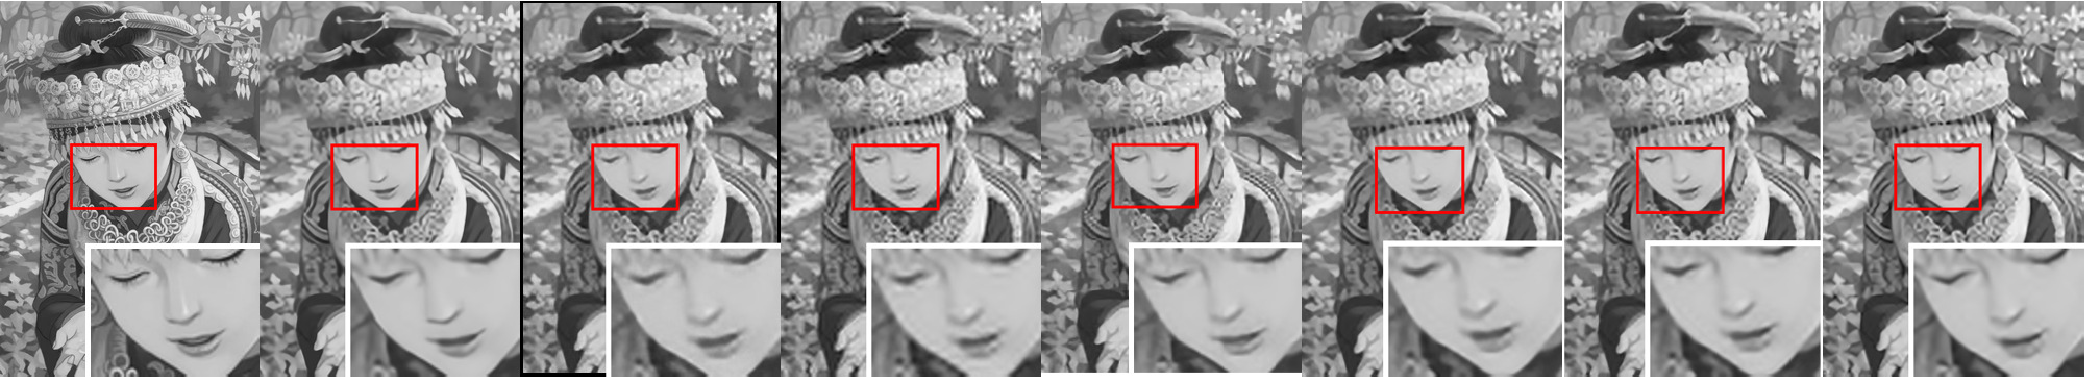
\includegraphics[width=1\textwidth]{3-4} }
\caption{Visual results of image super-resolution.
Images from left to right column are: High resolution image;
the recovered image of RED30, ARFL+, CSC, CSCN, NBSRF, SRCNN, TSE.}
\label{fig14}
\end{figure*}




\subsection{JPEG deblocking}

Lossy compression, such as JPEG, introduces complex compression artifacts,
particularly the blocking artifacts, ringing effects and blurring. In this
section, we carry out deblocking experiments to recover high quality images
from their JPEG compression. As in other compression artifacts reduction methods,
standard JPEG compression schemes of JPEG quality settings $q = 10$ and $q = 20$ in
MATLAB JPEG encoder are used. The LIVE1 dataset is used for evaluation, and we
have compared our method with AR-CNN \cite{DBLP:conf/iccv/DongDLT15}, SA-DCT
~\cite{DBLP:journals/tip/FoiKE07} and deeper SRCNN \cite{DBLP:conf/iccv/DongDLT15}.

The results are shown in Table \ref{table9}. We can observe that since the
Euclidean loss favors a high PSNR, our network outperforms other methods.
Compared to AR-CNN, the 30-layer network exceeds it by 0.37dB and 0.44dB on
compression quality of 10 and 20. Meanwhile, we can see that compared to
shallow networks, using significantly deeper networks does improve the deblocking performance.

\begin{table*}[htb!]
\centering
%
\caption{JPEG compression deblock: average PSNR results of LIVE1.}
\begin{tabular}{c|c c c c c c} \hline
              &SA-DCT   &Deeper SRCNN   &AR-CNN   &RED10   &RED20  &RED30           \\ \hline
  Quality $=10$  &28.65  	&28.92          &28.98    &29.24   &29.33  &\textbf{29.35}  \\ \hline
  Quality $=20$  &30.81  	&-              &31.29    &31.63   &31.71  &\textbf{31.73}  \\ \hline
\end{tabular}
\label{table9}
\end{table*}



\subsection{Non-blind deblurring}

We mainly follow the experimental protocols as in ~\cite{DBLP:conf/nips/XuRLJ14} for
evaluation of non-blind deblurring. The performance on deblurring ``disk", ``motion"
and ``gaussian" kernels are compared, as shown in Table \ref{table10}. We generate
blurred image patches with the corresponding kernels, and train end-to-end
mapping with pairs of blurred and non-blurred image patches. As we can see from the results,
our network outperforms those compared methods with significant improvements. Figure~\ref{fig17} shows some visual comparisons.
We can observe from the visual examples
that our network works better than the compared methods on recovering the image details,
as well as achieving visually more appealing results on low frequency image contents.


\begin{table*}[htb]
\centering
%
\caption{PSNR results on non-blind deblurring.}
\begin{tabular}{c|c c c c c c} \hline
  kernel tpye  &Krishnan~et al.~\cite{DBLP:conf/nips/KrishnanF09}
  &Levin~et al.~\cite{DBLP:journals/tog/LevinFDF07}
               &Cho~et al.~\cite{DBLP:conf/iccv/ChoWL11}
               &Schuler et al.~\cite{DBLP:conf/cvpr/SchulerBHS13}
               &Xu~et al.~\cite{DBLP:conf/nips/XuRLJ14}    &RED30	\\ \hline
  disk    	&25.94  &24.54  &23.97  &24.67  &26.01  &\textbf{32.13}	\\ \hline
  motion    &30.34  &37.80  &33.25  &-      &-      &\textbf{38.84}	\\ \hline
  gaussian  &27.90  &32.34  &30.09  &30.97  &-      &\textbf{34.49}	\\ \hline
 \end{tabular}
\label{table10}
\end{table*}




\begin{figure*}
\centering
\subfigure{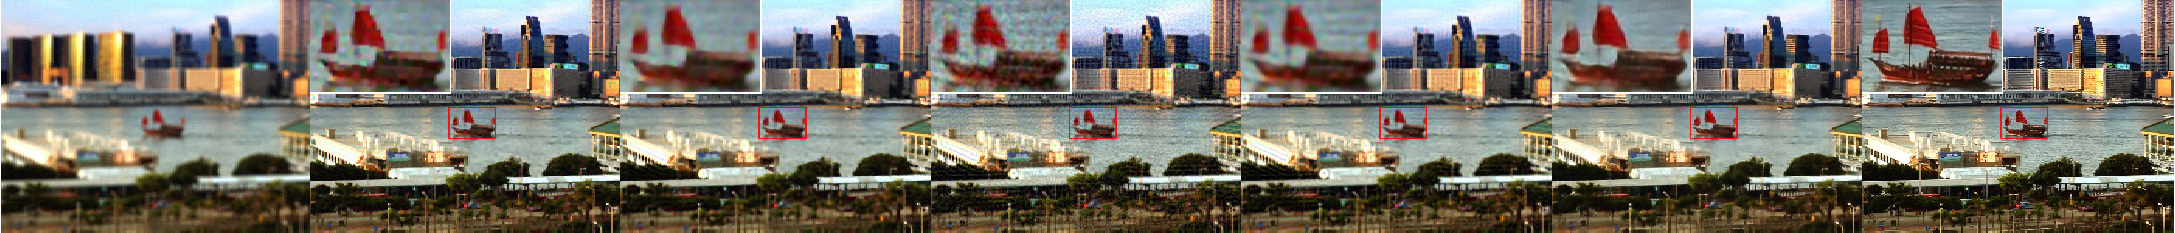
\includegraphics[width=1\textwidth]{deblur1} }
\subfigure{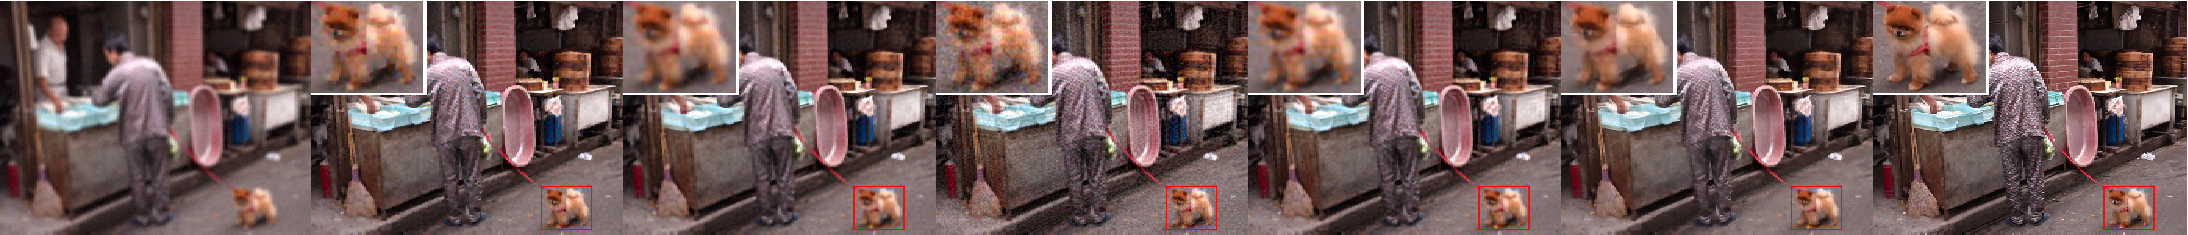
\includegraphics[width=1\textwidth]{deblur2} }
\subfigure{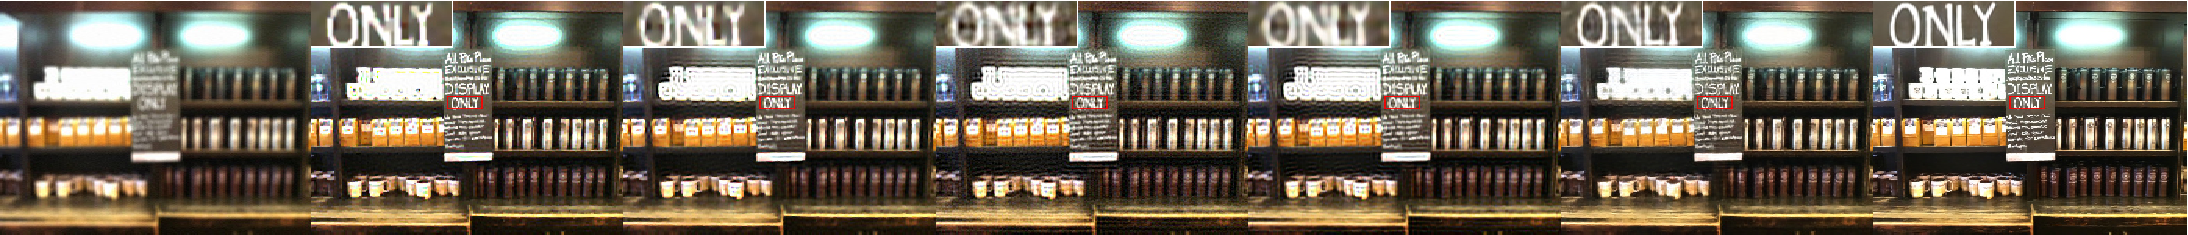
\includegraphics[width=1\textwidth]{deblur3} }
\caption{Visual comparisons on non-blind deblurring. Images from left to right are:
blurred images, the results of Cho~\cite{DBLP:conf/iccv/ChoWL11},
Krishnan~\cite{DBLP:conf/nips/KrishnanF09}, Levin~\cite{DBLP:journals/tog/LevinFDF07},
Schuler~\cite{DBLP:conf/cvpr/SchulerBHS13}, Xu~\cite{DBLP:conf/nips/XuRLJ14}
and our method.}
\label{fig17}
\end{figure*}




\subsection{Image inpainting}
In this section,
we conduct text removal for experiments of image inpainting. Text is added
to the original image from the LIVE1 dataset  with font size of 10 and 20.
We have compared our method with FoE ~\cite{DBLP:journals/ijcv/RothB09}. For our model,
we extract image patches with text on them and learn a mapping from them to the
original patches. For FoE, we provide both images with text and masks indicating
which pixel is corrupted.

The average PSNR and SSIM for font size 10 and 20 on LIVE are:
38.24dB, 0.9869 and 34.99dB, 0.9828 using 30-layer RED-Net, and they are much
better than those of FoE, which are 34.59dB, 0.9762 and 31.10dB, 0.9510. For scratch
removal, we randomly draw scratch on the clean image and test with our network and FoE. The PSNR and SSIM for our network are 39.41dB and 0.9923, which is much better than 32.92dB and 0.9686 of FoE.

Figure \ref{fig15} shows some visual comparisons of our method between FoE. We can
observe from the examples that our network is better at recovering text, logos,
faces and edges in the natural images. Looking on the first example, one may wonder
why the text in the original image is not eliminated. For traditional methods
such as FoE, this problem is addressed by providing a mask, which indicates the
location of corrupted pixels. While our network is trained on specific distributions
of corruptions, i.e., the text of font sizes 10 and 20 that are added.
It is equivalent to distinguishing corrupted and non-corrupted pixels of different distributions.

\begin{figure*}
\centering
\subfigure{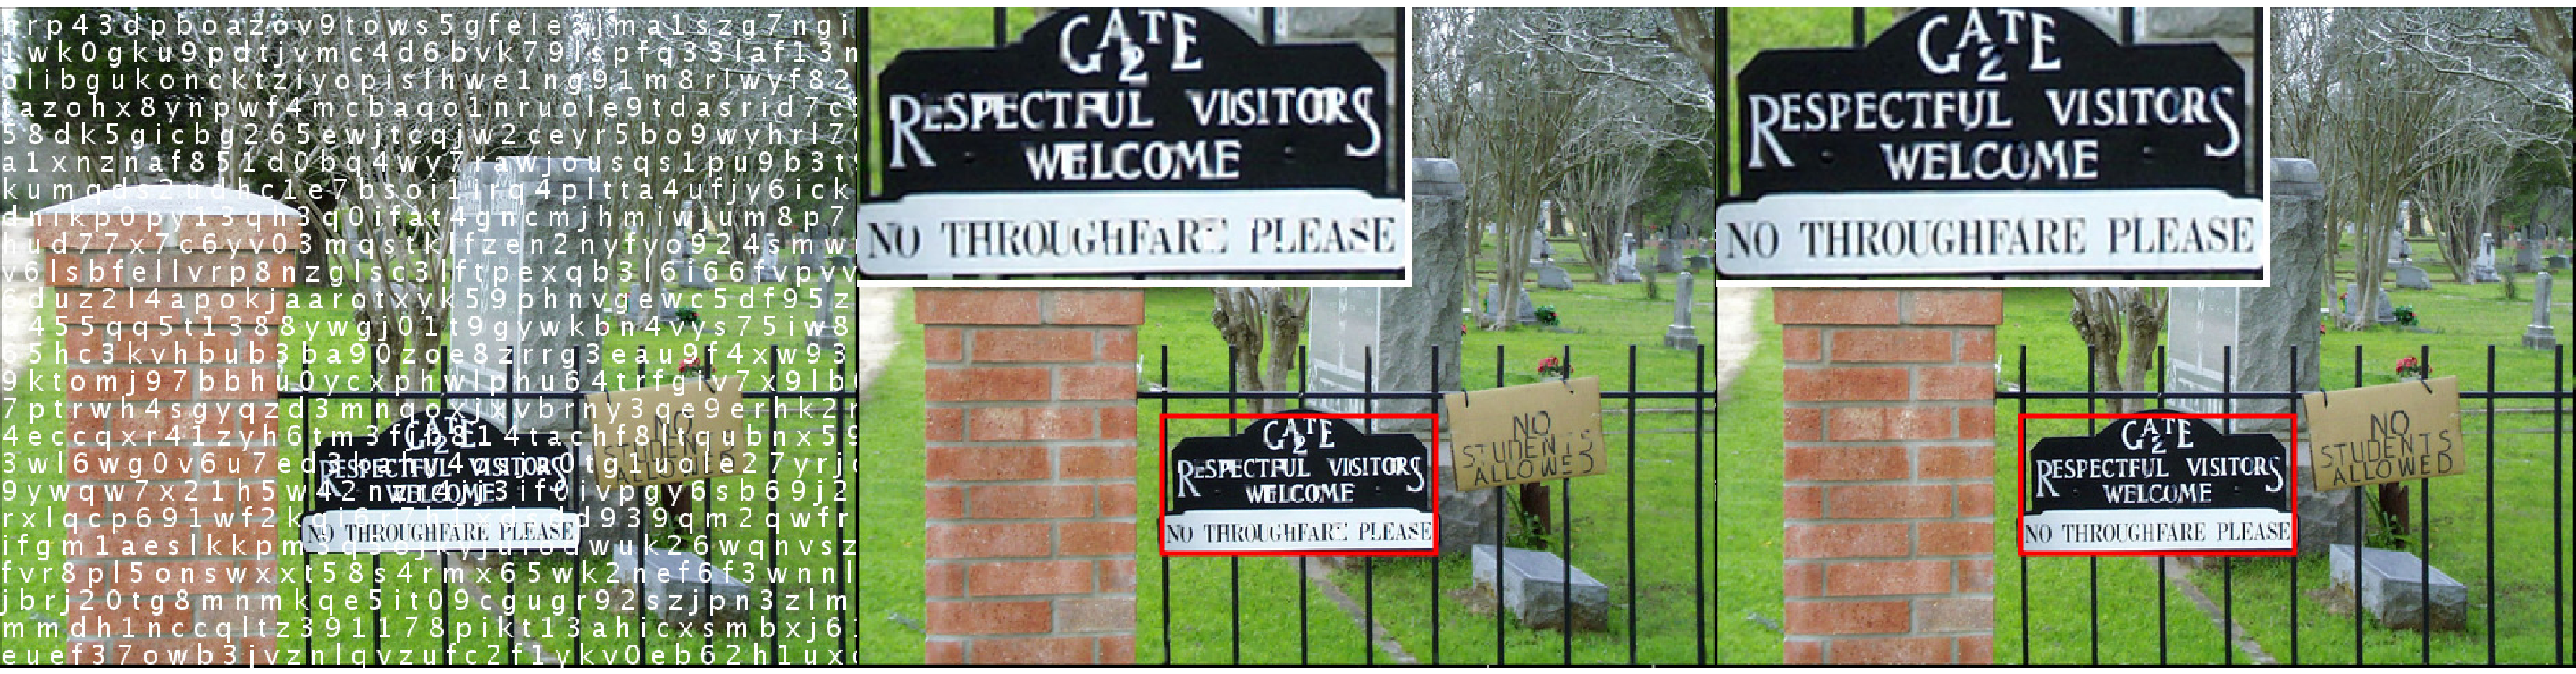
\includegraphics[width=0.9\textwidth]{inpainting_1} }
\subfigure{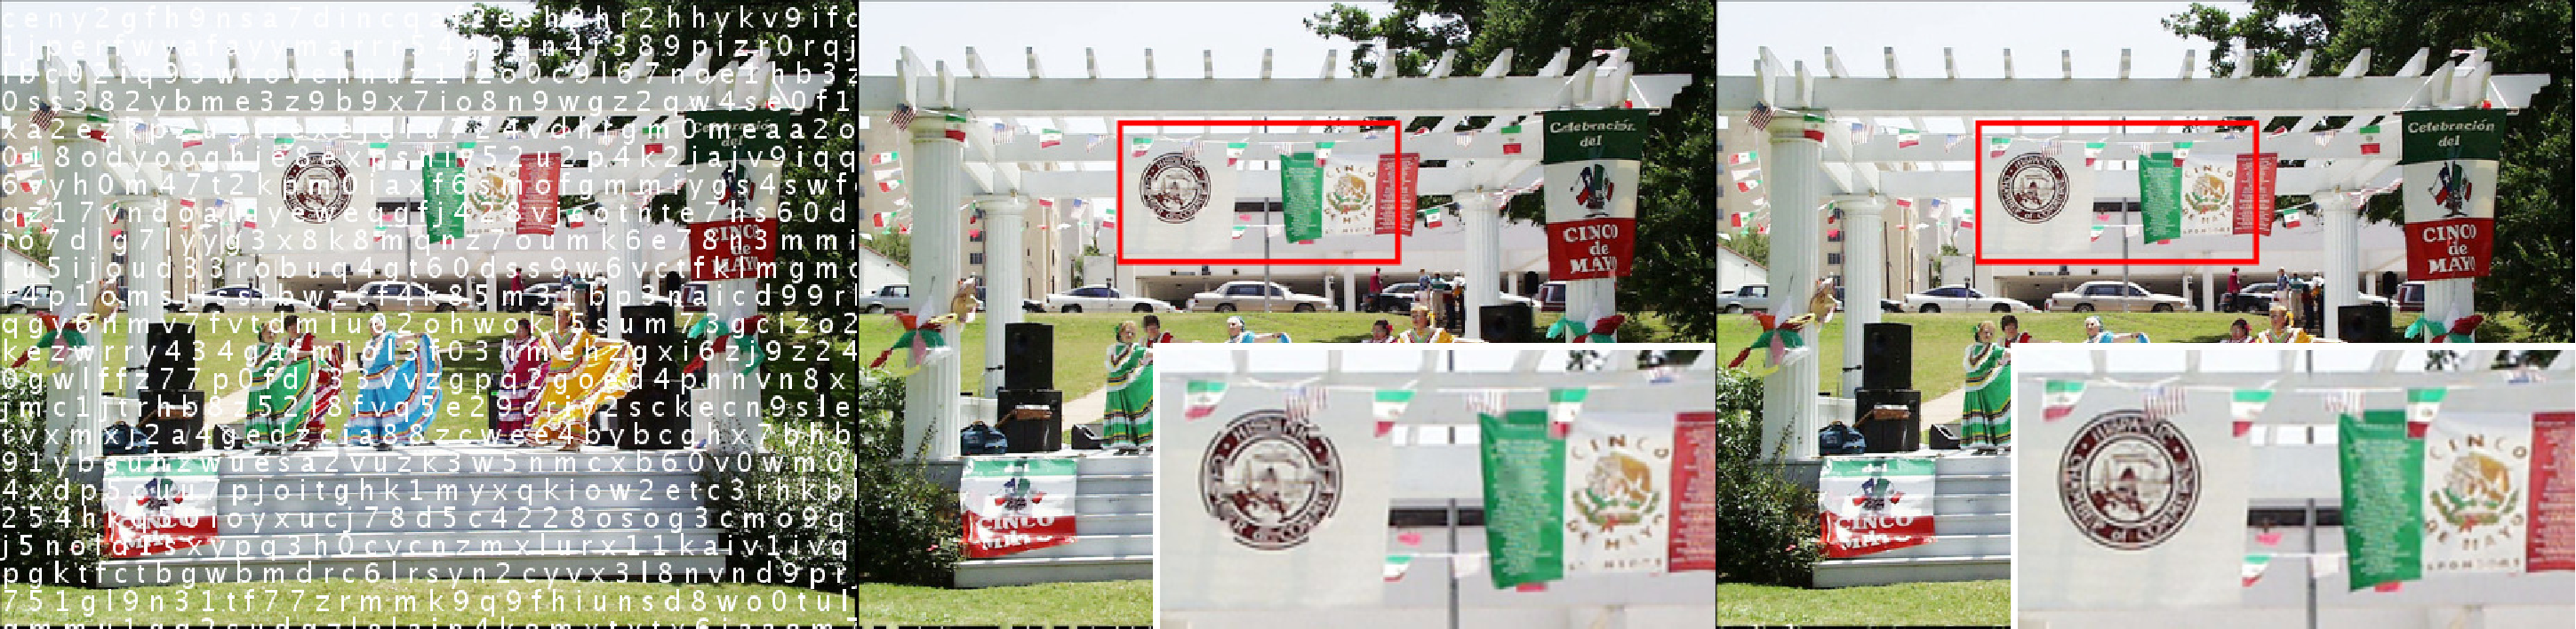
\includegraphics[width=0.9\textwidth]{inpainting_2} }
\subfigure{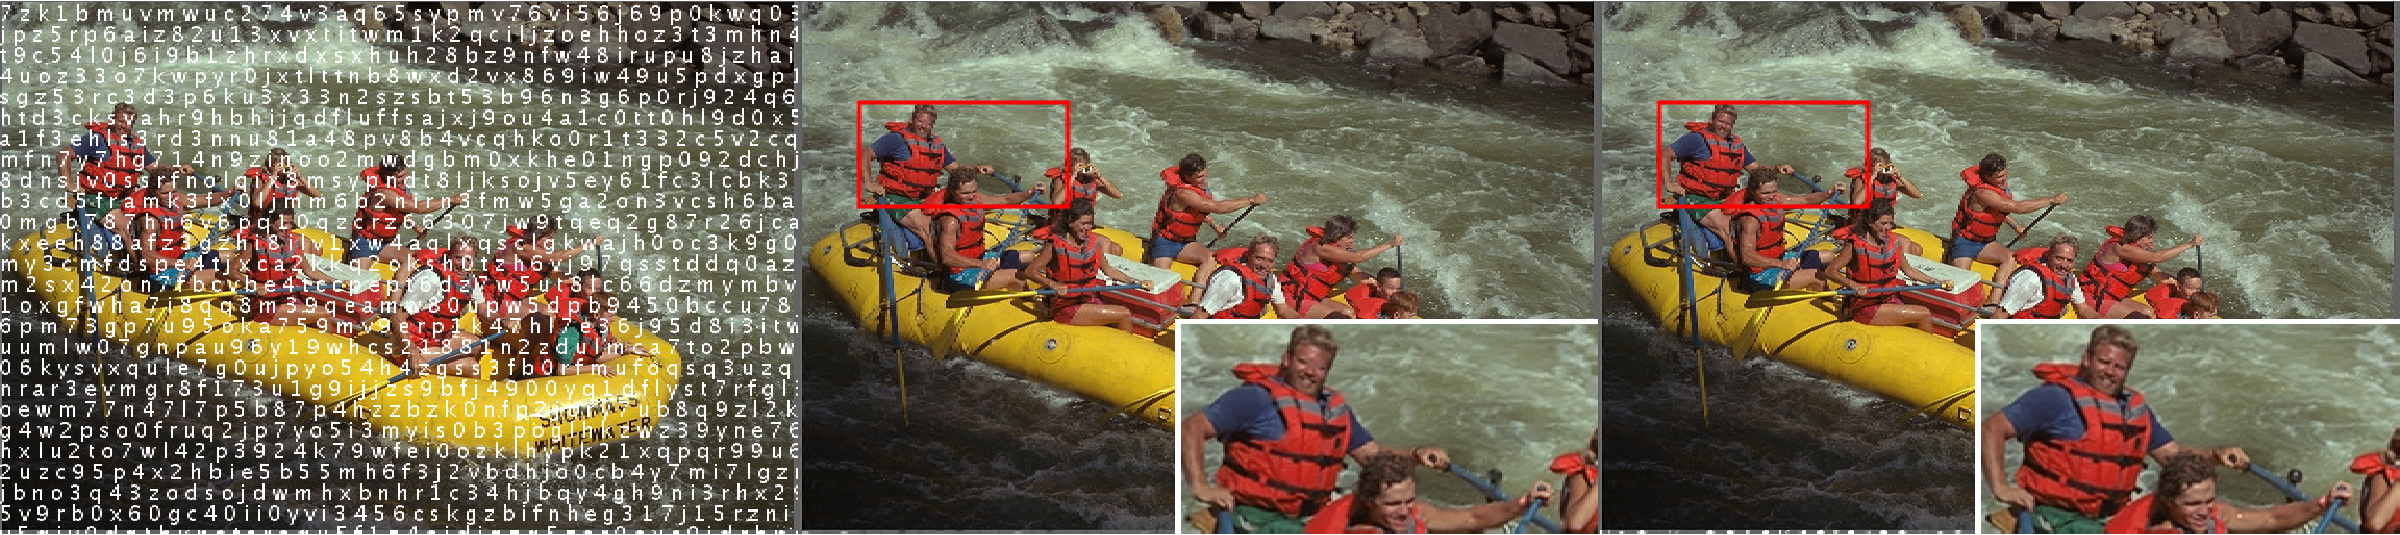
\includegraphics[width=0.9\textwidth]{inpainting_3} }
\subfigure{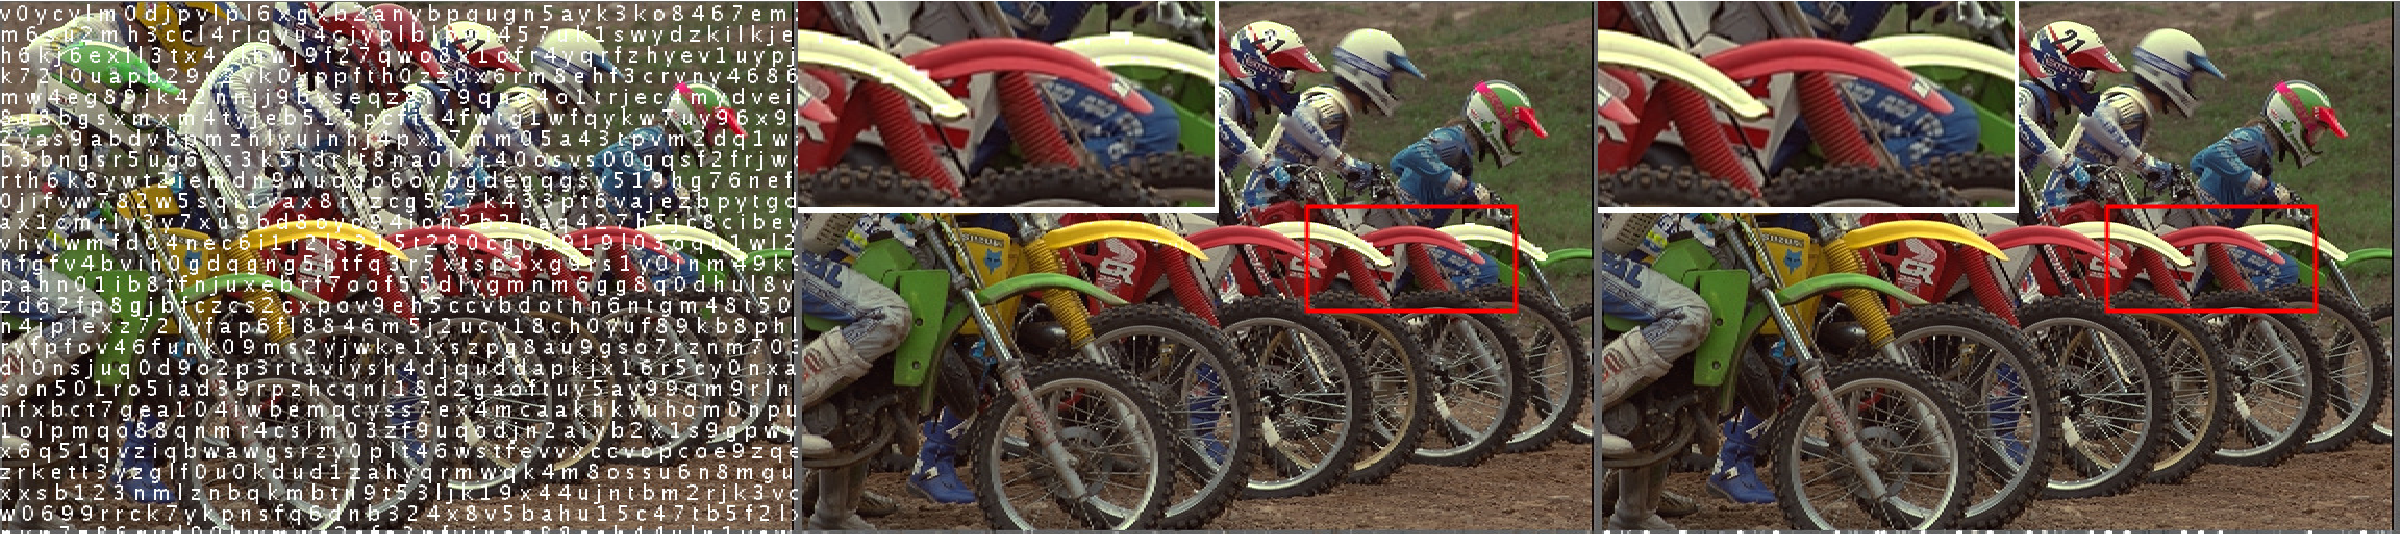
\includegraphics[width=0.9\textwidth]{inpainting_4} }
\subfigure{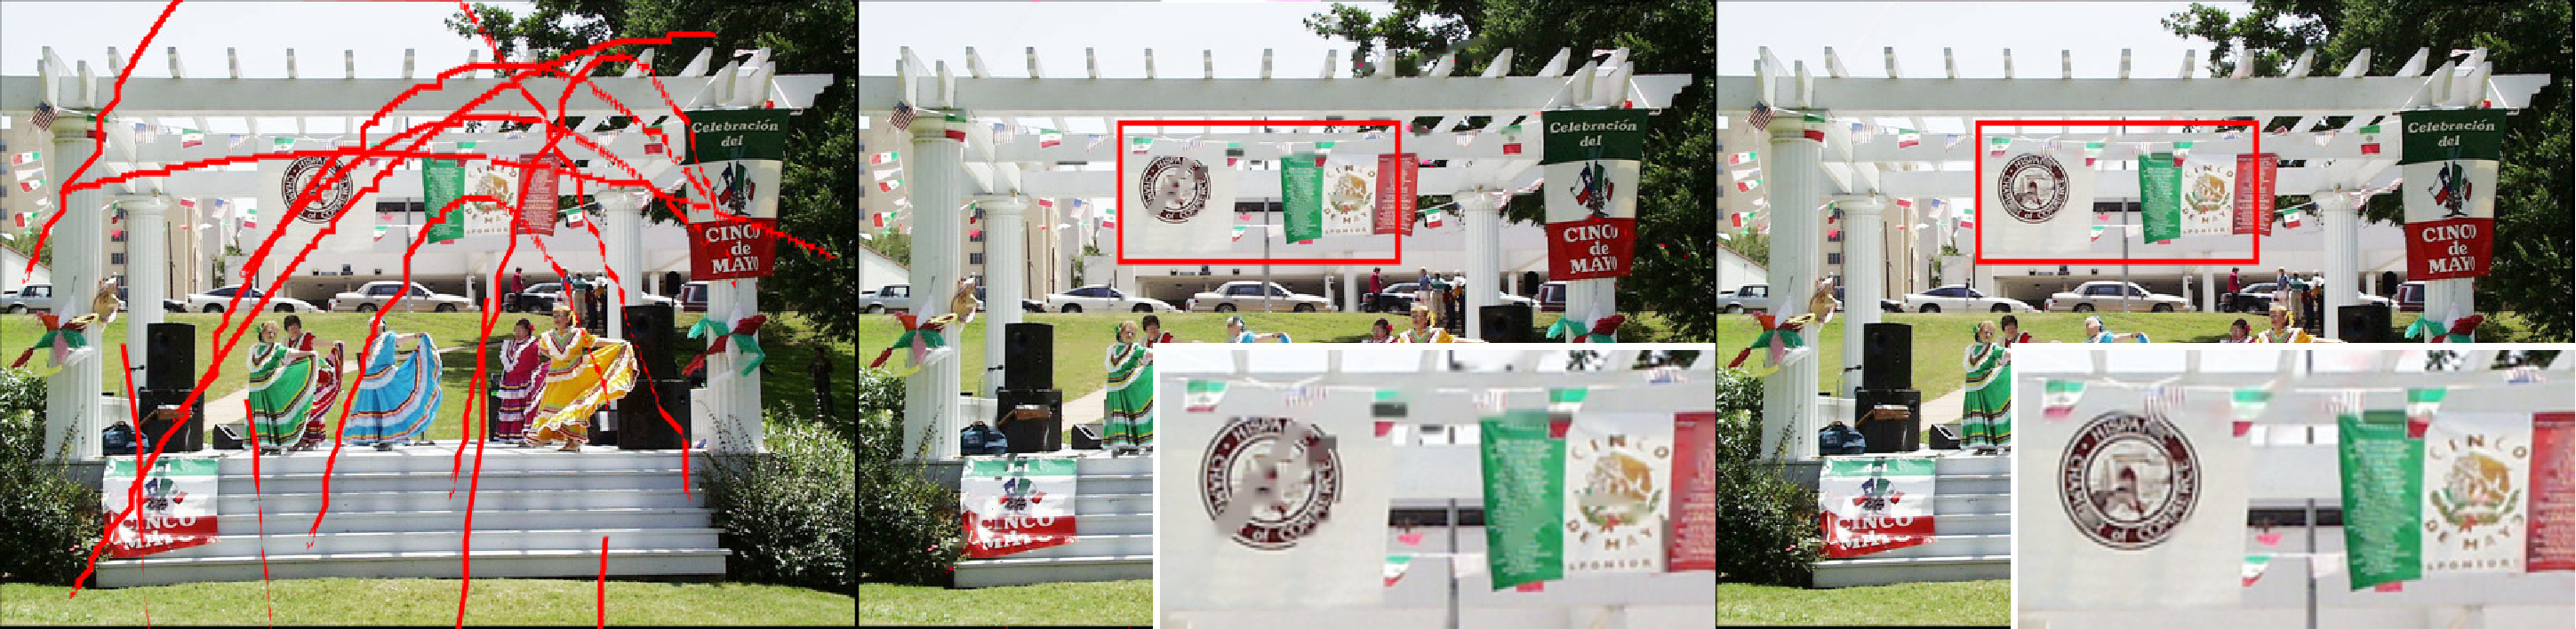
\includegraphics[width=0.9\textwidth]{inpainting_5} }
\caption{Visual results of our method and FoE. Images from left to right are:
Corrupted images, the inpainting results of FoE and the inpainting results of our method. We see better recovered details as shown in the zoomed
patches.}
\label{fig15}
\end{figure*}



